\section{Models}
\begin{figure}[h]
  \centering
  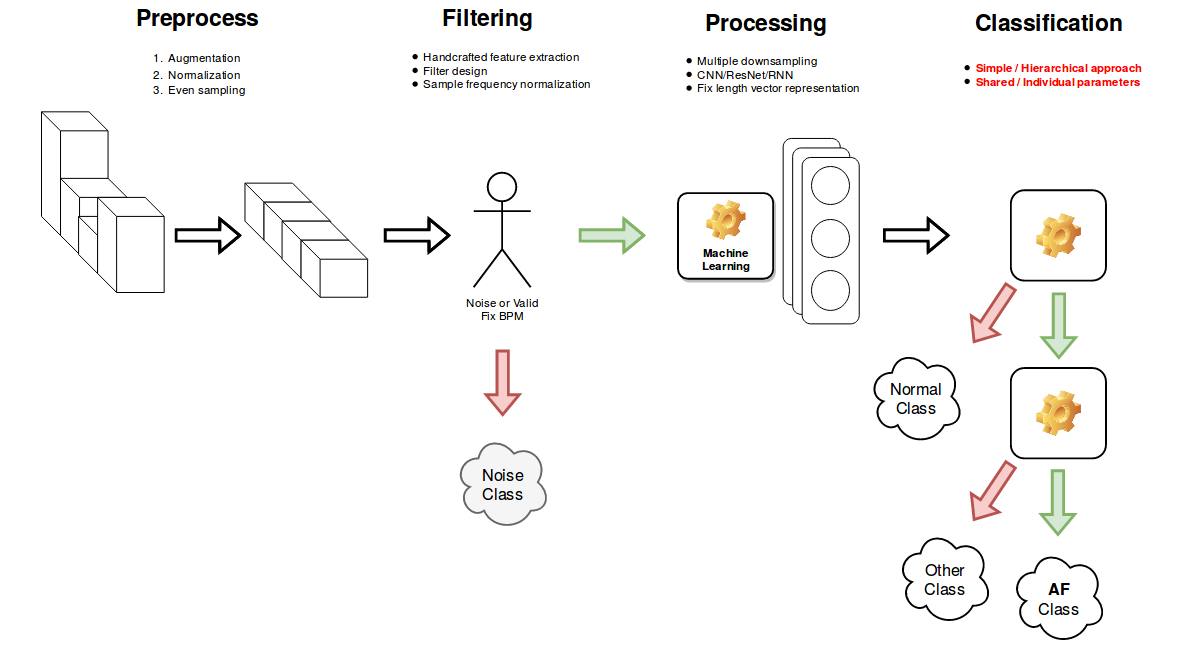
\includegraphics[width=.8\textwidth]{method}\label{fig:method}
  \caption{We believe that our best chance to classify samples properly is that we learn how to separate \textit{valid} and \textit{noisy} data from one-another --- since the model will not be forced then to be able to recognize delicate patterns which could indicate heart failure along with harsh noise patterns. In order to avoid overfitting on the small train set of a few hundred samples, instead simply training a binary classifier network, we are working hard to filter these noisy samples by other handcrafted approaches. Next, the sample should be categorized as a healthy or an unhealthy ECG. As a final step, we are training a network to distinguish atrium fibrillation from other ill ECG. During the training process the different part of the model are trained separately only on their own domain, and after descending below a certain error rate, we assemble the model.}
\end{figure}

As mentioned before, we intended to exploit the late success of neural networks that offers a plenty of methods and architectures --- and a few rule of thumbs to keep in mind when preparing the blueprint.
Currently we are experimenting with hierarchical classification models.~\ref{fig:method}
At the time of writing I will describe the main building blocks we have tried before, and present the baseline our recent tests are based upon.
My role in the group is to implement and maintain the deep learning back-end, also to integrate the hand crafted features, and carry out experiments and evaluate them to determine which combination leads to the most successful architecture.

\paragraph{Variable length representation.}
First of all, we have to deal with time dependency. Since we cannot determine how long the samples will be, nor describe a time frame that would fit every relevant pattern, we have to project somehow the sample into a fixed dimensional space. In order to preserve important information by the projection we can separate samples into clusters by previously extracting features which describes best the data. These values are usually time dependent pattern fitting maps.

\begin{figure}
  \centering
  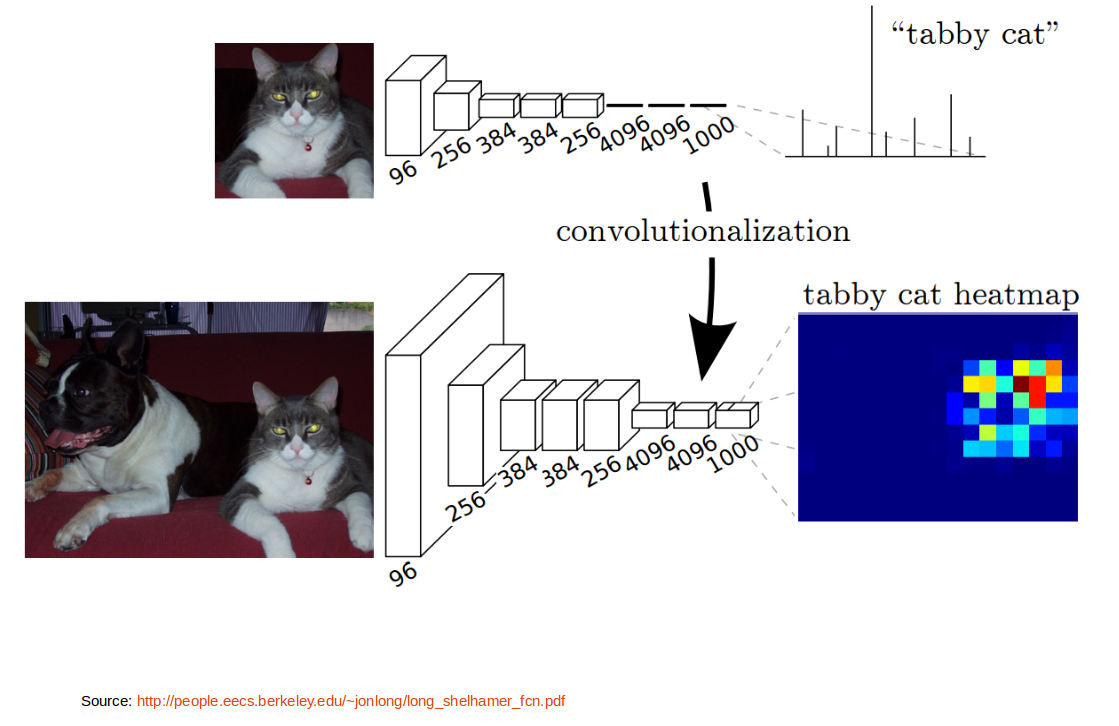
\includegraphics[width=.8\textwidth]{FCN}\label{fig:FCN}
  \caption{Semantic segmentation (bottom) uses the feature extractors from VGG (top), by simply reshaping the fully connected layers into convolutions with local receptive fields. We expect the same behavior when training convolutional networks on one dimensional time series. Image credits~\cite{Long_2015_CVPR}}
\end{figure}

Based on the fact that hierarchical feature extractors such as the LeNet~\cite{lecun1995convolutional}, and the VGG\cite{VGG} are easily trained, reliable, and can be easily restructured for transfer learning purposes~\cite{transfer learning} I decided to re-implement the Fully Convolutional Network~\cite{Long_2015_CVPR} paradigm in one dimension motivated by the following works~\cite{mittelman2015time, langkvist2014review}.
The actual convolutional layers of our FCN models are following the pattern:
\begin{center}
  \begin{equation}
    \begin{split}
      c &= \mathbf{K} \ast x\\
      b &= BatchNorm(c)\\
      h &= ReLU(b)\\
      y &= AvgPool_w(h)
    \end{split}
  \end{equation}
\end{center}

Where BatchNorm is described in~\cite{batchnorm}, and ReLU is the rectified linear unit (nonlinear) activation function, and $w$ indicates the window size of the pooling operation (the stride was set to the same value as well).
Hyper-parameters of this convolutional layer are hidden in the dimensions of  $\mathbf{K}\rightarrow$ \texttt{[IN, OUT, k]}, where \texttt{IN} is fixed, \texttt{OUT} represents how many feature maps will be created by the convolution operation, and \texttt{k} is how large the kernel will be, i.e. how large the receptive field will this layer have on $x$.
These layers were assembled in the depicted manner on \ref{fig:baseline} (top row).

\begin{figure}
  \centering
  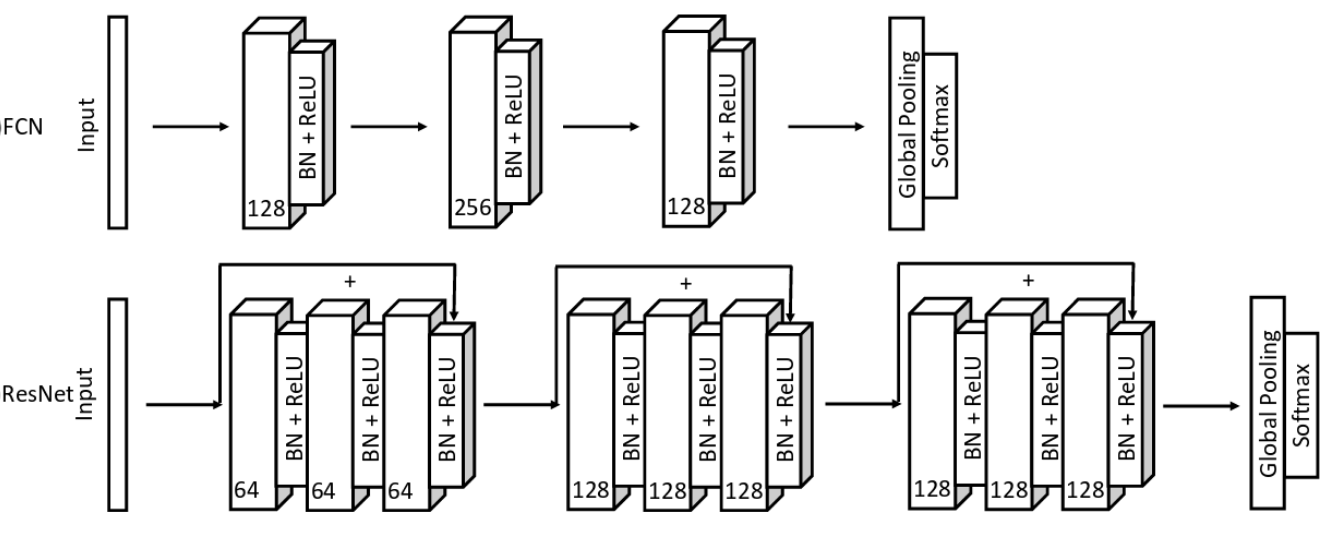
\includegraphics[width=\textwidth]{baseline}\label{fig:baseline}
  \caption{Image credits~\cite{wang2016time}}
\end{figure}

We also began experimenting with Deep Residual Networks (ResNets)~\cite{he2016deep}, suggested by~\cite{wang2016time}.
The basic idea is simple: we concatenate several of the above mentioned FCNs after each other, while stabilizing the gradient flow by adding the convolutional blocks' input to their output.
However the interpretations of how deep residual networks actually work so well are not clear, an excellent article on this topic \cite{resnet-ensembles},
Oversimplifying, we could say that now each FCN blocks in the model are not responsible for detecting every feature, just as shallow networks to work together as different ensembles, which allows us to increase the overall capacity of the model.

\paragraph{Fixed length representation.}
Once every filters have been evaluated in the end we can use different approaches: to take the weighted norm or mean of the filtered signal to represent each pattern's presence in the input signal or we can use techniques that have been proven to be successful in natural language processing tasks, the recurrent neural networks.
Our first attempt was using Long Short Term Memory network (LSTM)~\cite{hochreiter1997long, malhotra2015long} shortly after switched to its modified version Gated Recurrent Unit network (GRU)~\cite{chung2014empirical}, but we experienced that the network was not capable even to overfit the train set, and achieve a satisfactory error rate.
Due to the large number of task specific hyper-parameters in LSTMs and GRUs the search space would exponentially increase, so we decided to continue experimenting with simply reducing the feature map to a single scalar value by mean averaging the activation through time of the feature extractors.

\paragraph{Augmentation and transfer learning.}
Despite the initial difficulties with RNN, I began to experiment as an offspin project to apply RNN as a time series predictor, training it to predict the following $N$ values of the measurements based on the previous parts of the sample. I believe that this model can be reused to initialize training classifier recurrent networks, instead of random initialization.
On the other hand, by feeding back the network its own predictions we could produce data \ref{fig:rnn-aug}. The network in this case would function as some sort of "language model"~\cite{lang-model} of ECG signals - and if trained properly, i.e. on a single class, it would output labeled, yet totally artificial samples, which could be used as augmented training data as well.

\begin{figure}
  \centering
  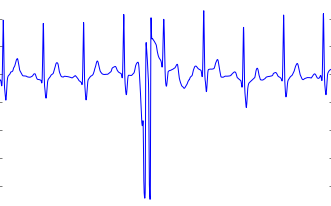
\includegraphics[width=\textwidth]{rnn-aug}\label{fig:rnn-aug}
  \caption{Artificial sample produced by an LSTM trained to predict and continue original ECG samples. In this case the network functions as some sort of language model of ECG. Among many samples, professionals could not tell whether samples produced by this method were artificial or taken from the original training set. Truth on being told, after further analyzes they could detect artifacts, still some said that a very ill patient could produce the same samples. \textbf{TODO: provide more samples, or an original sample to let the reader decide which is which.}}
\end{figure}

\paragraph{Classification}
After extracting the most relevant time features from the sample, and reduced it to a fix length feature vector, the model has to separate the feature space with respect to the classes.
A basic approach is to apply logistic regression where each feature dimension is taken into account and weighted to determine each class (by dissecting the feature space with hyper-planes).
As a result a four dimensional vector $[0, 1]^4$ is produced, where each dimension represents the confidence of the network whether the sample is belonging to the corresponding class or not. The output is then normalized with the softmax function to give a confidence distribution over the classes:
\begin{equation}
p_i = \frac{\exp(y_i)}{|\exp(y)|_1}
\end{equation}
We also tried applying Multiple Layer Perceptrons (MLP)~\cite{girshick2014rich}, on the top of these features, however the results show that the model is less likely to collapse during training due to falling in a local minimum.
